As said in Chapter 1, the proposed strategy to solve the audio \gls{sr} task is based on an hybrid architecture that combines both \gls{tfnet} \cite{lim2018time} and \gls{tfilm} \cite{birnbaum2019temporal} methods. In order to describe our system, a previous analysis of the two models from which the proposed one derives needs to be done. For this reason, both \gls{tfnet} and \gls{tfilm} approaches are described in paragraphs \ref{tfnet} and \ref{tfilm}, respectively. \\
All methods for audio \gls{sr} that are presented in this chapter derive from a mathematical formulation that treats this task as a pure regression problem.
As stated in paragraph \ref{problem_formulation}, the goal of the model is to characterize the conditional distribution $p(y|x)$ of a \gls{hr} sequence given its \gls{lr} input. Therefore, the point-estimate output results in a sequence $\hat{y} = f_{\theta}(x)$ of real values. This formulation naturally leads to the least-squares optimization problem of the form:
\begin{align}\label{eq:regression_formulation}
	\begin{array}{c}
		\min _{\theta} \sum_{i}\left\|f_{\theta}(x_{i})-y_{i}\right\|_{2}^{2}
	\end{array}
\end{align}
where $\|.\|$ denotes the norm function, $x_i, y_i$ are training examples such that $\mathcal{D} = \{x_i, y_i\}_{i = 1}^n$ and $f_{\theta}$ is the \gls{dl} model parametrized by $\theta$. As a natural consequence of this setting, the objective function of this work can be defined as:
\begin{align}\label{eq:regression_loss}
	\begin{array}{c}
		\ell(\mathcal{D})=\frac{1}{n} \sqrt{\sum_{i=1}^{n}\left\|y_{i}-f_{\theta}\left(x_{i}\right)\right\|_{2}^{2}}
	\end{array}
\end{align}
In other words, artificial \gls{bwe} can be seen as a structured regression task, where the goal is to minimize the difference between the model point estimation and the target sequence. \\
The problem can be tackled by deep neural network architectures, that have enough capacity to perform non-linear regression. Indeed, many levels of non-linearities allow them to represent a complex non-linear regression function that maps \gls{lr} input data to \gls{hr} audio frames. Therefore, all \gls{dl} systems presented in this chapter are trained in order to minimize the metric given in Equation \ref{eq:regression_loss}. \\
Another common factor shared by all of these audio \gls{sr} methods is that the source input is pre-processed with a  a cubic B-spline upscaling in order to ensure \gls{lr}/\gls{hr} signals are of the same length. This operation has multiple advantages. On one hand, it allows to have a baseline to compare the results of \gls{dl} models. On the other hand, since this operation is included in the processing pipeline, it is possible to exploit it by the use of residual connections to link the input and the output series. This solution allows to speed up the required training time, because the model  $f_{\theta}$ is facilitated by having to estimate only the difference between the \gls{lr} source and the target \gls{hr} signal. This and all other pre-processing operations are discussed in detail in Chapter ~\ref{chap:exp_results}. \\
It is important to point out that, due to computational limitations, it is not possible, in this work, to propose and train a new model that has the same number of parameters than \gls{tfnet} and \gls{tfilm}. Therefore, results reported in the two model papers can not be used to make comparisons between different architectures. In fact, model comparisons must be performed in fair contexts, i.e., by training models with approximately the same number of parameters. For this reason, \gls{tfnet} and \gls{tfilm} models are
reduced in size and, subsequently, re-trained so that they can be compared with the proposed architecture under the same conditions. \\
This chapter aims not only to provide a clear idea of the original configurations of the models, but also to describe the changes made to reduce dimensionality. Therefore, in the paragraphs \ref{tfnet} and \ref{tfilm}, the models \gls{tfnet} e \gls{tfilm}, respectively, are described in their original configurations. Then, in the paragraph \ref{implementation_details}, all
details related to the implementation of the models, and the changes made to the original configurations are thoroughly described.

\section{TFNet} \label{tfnet}
Time-Frequency Network, proposed by Lim, Yeh \textit{et  al.}\cite{lim2018time}, is the first model in literature that addresses the problem of audio \gls{sr} by operating in both time and frequency domain. In the paper, authors highlight the origin of their intuition. “At the first glance, modeling in both frequency and time domain seems like a redundant representation; From Parseval’s theorem the $\ell_{2}$ difference of prediction error, whether in the frequency or time domain is exactly the same. However, regression from \gls{lr} to \gls{hr} in time or frequency domain solves a very different problem. In the time domain, it is analogous to the image super-resolution task, mapping \textit{audio patches} from \gls{lr} to \gls{hr}. On the other hand, \gls{sr} in the frequency domain is analogous to the \textit{semantic image inpainting} task (\gls{bwe} in spectral domain can be viewed as image inpainting of spectrograms) \cite{pathak2016context},\cite{yeh2017semantic}”. \\
\begin{figure}[H]
	\begin{center}
		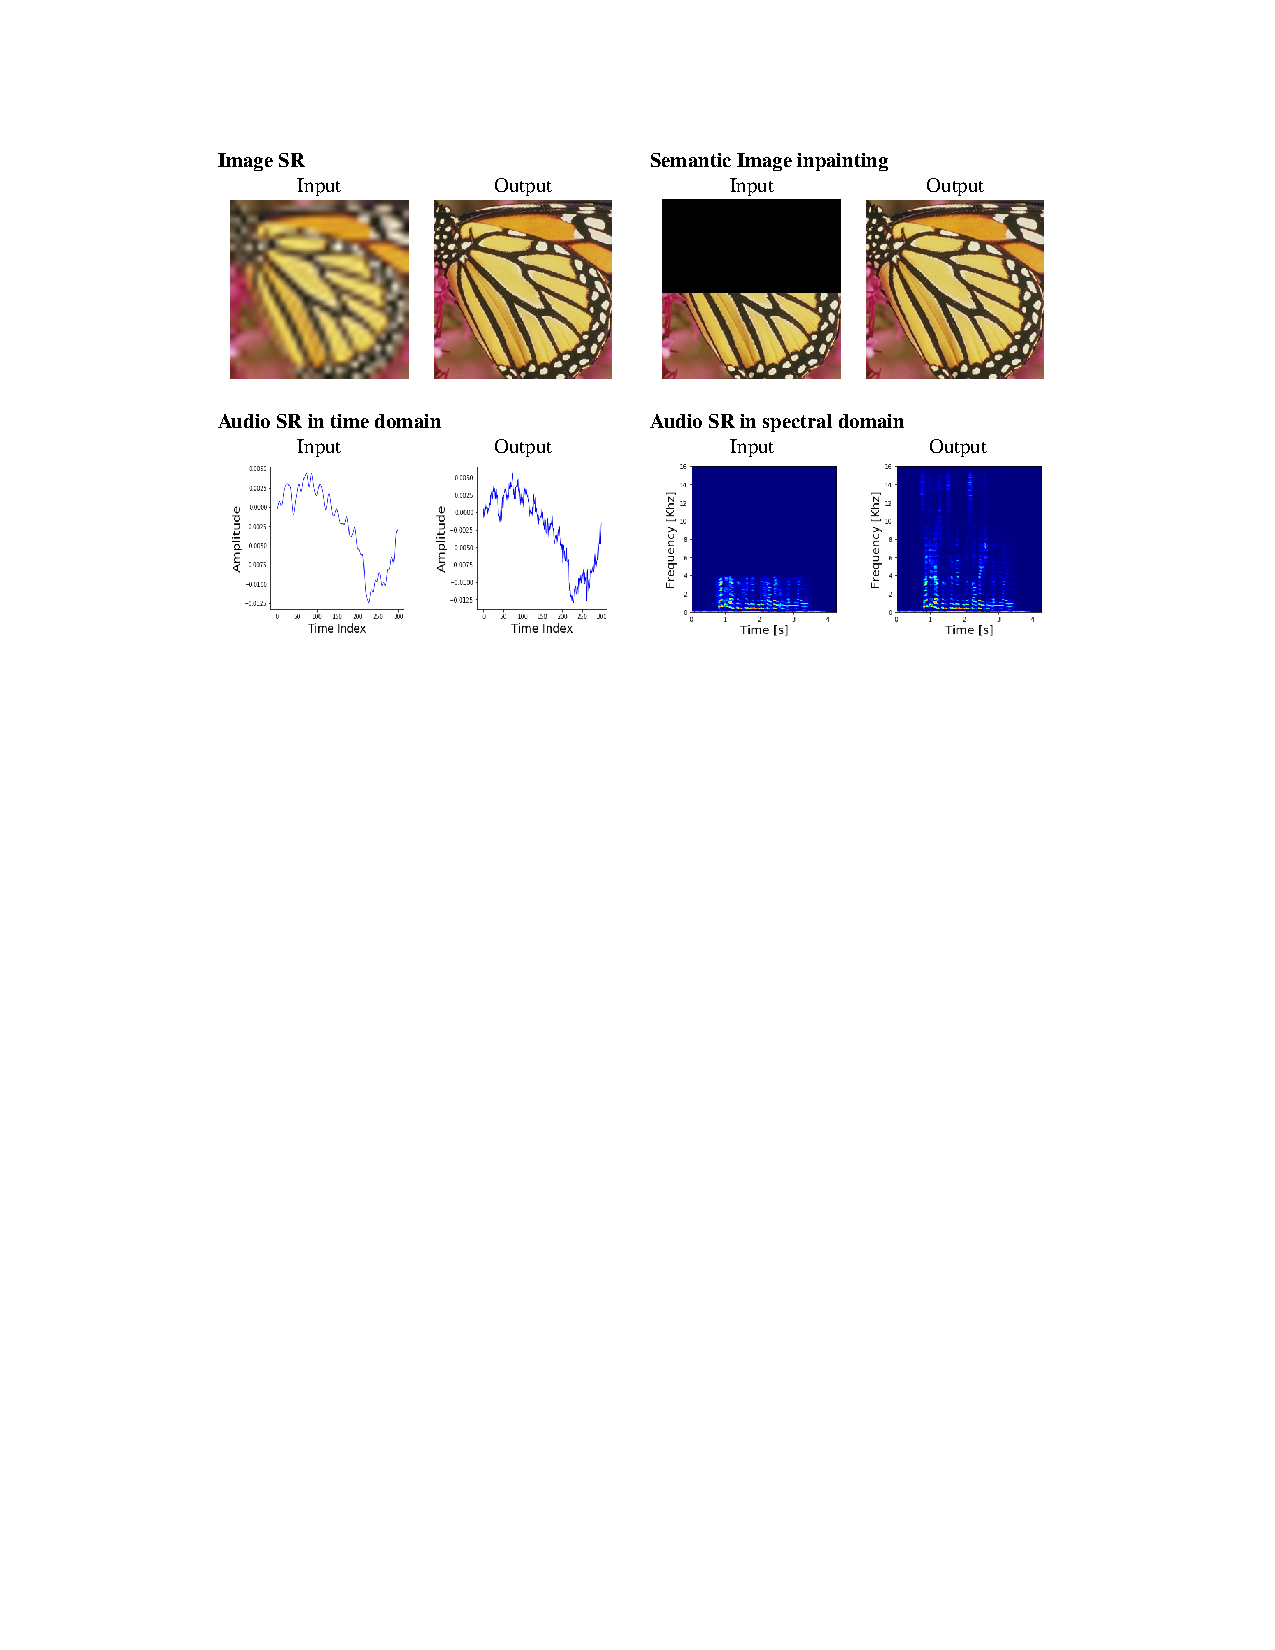
\includegraphics[scale=1.11]{img/tfnet_intuition.pdf}
		\captionsetup{margin=2cm}
		\caption{\textit{Top row}: Examples of image \gls{sr} and semantic image inpainting reconstruction. \textit{Bottom row}: Illustration of the input/output for audio \gls{sr} in time and frequency domain. From \cite{lim2018time}.}
		\label{fig:tfnet_intuition}
	\end{center}
\end{figure}
\noindent Figure ~\ref{fig:tfnet_intuition} sums up the close relationship that links audio \gls{sr} in time domain with image \gls{sr}, and audio \gls{sr} in frequency domain with image inpainting. \\
Based on these considerations, authors propose a system made of two main branches: one which models signals in the spectral domain, while the other branch explicitly models the reconstruction in time domain. \\
More specifically, \gls{tfnet} is a fully differentiable network that estimates, for a given \gls{lr} input $x$, the \gls{hr} audio reconstruction $\hat{z}$, and the \gls{hr} spectral magnitude $\hat{m}$. The last layer of the model, called \textit{Spectral Fusion Layer}, computes Fourier transform operations in order to combine $\hat{z}$ and $\hat{m}$ in a unique output $\hat{y}$. \\
A brief overview of the overall pipeline of the model architecture is provided in Fig. ~\ref{fig:tfnet_pipeline}. As we can see, the time-domain branch processes the signal through the "Slim AudioUNet" that is a fully convolutional component, explained in detail in \ref{audiounet}. The frequency branch performs more operations during the system processing: first, a \gls{dft} on the sequence is computed to pass from one domain to another. It is well known that when the \gls{dft} is performed on purely real input, such as audio signals, negative phase components are redundant and can be discarded. This is because the \gls{dft} of a real signal is Hermitian-symmetric, i.e. negative-frequency terms can be obtained from the corresponding positive terms. Therefore, given the \gls{lr} input signal $x$ of length $T_1$, only $\frac{T_1}{2} + 1$ components are taken into account: the zero-frequency term (DC component) followed by the $\frac{T_1}{2}$ positive-frequency terms. These $\frac{T_1}{2}$ values are then processed through the "Spectral Replicator" and "Slim AudioUNet", while the zero-frequency term pass directly through the network. A final concatenation operation is  applied in order to combine the DC component with the processed positive-frequency terms. \\
All the details concerning architectural components not yet presented, such as "Slim AudioUNet", "Spectral Replicator" and "Spectral Fusion Layer", are thoroughly studied in the next paragraphs. 

\begin{figure}[!htb]
	\begin{center}
		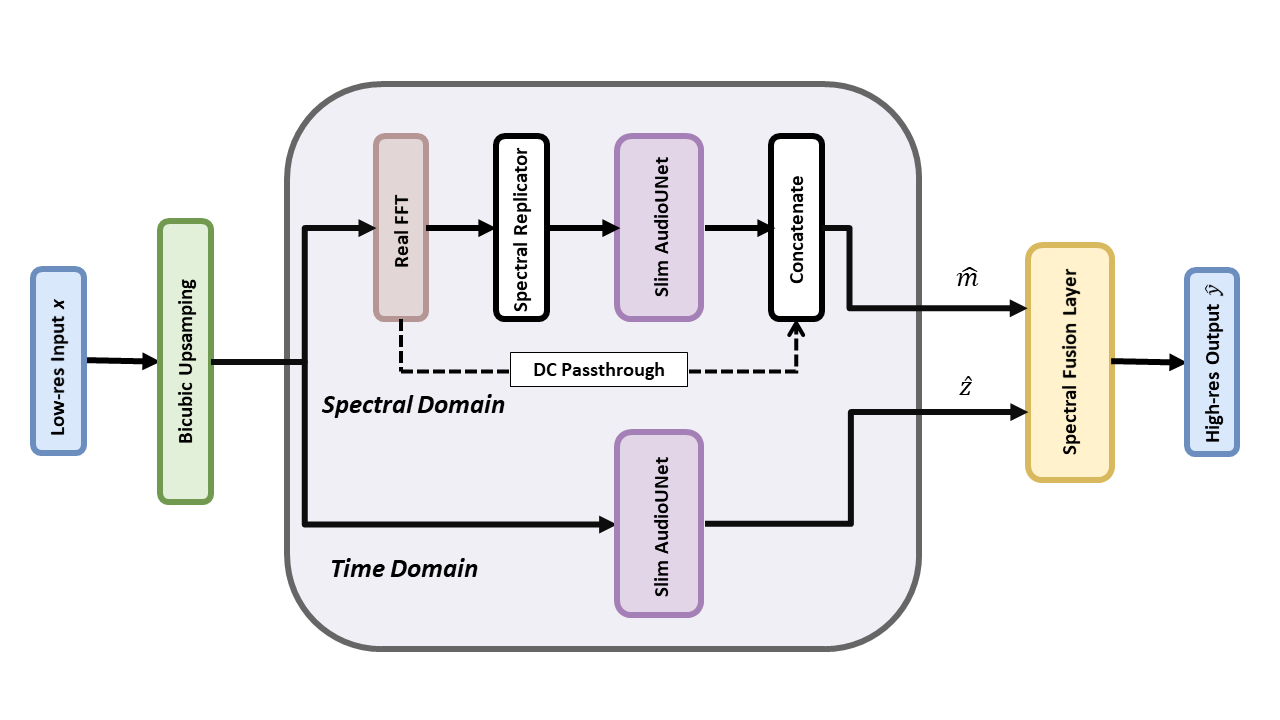
\includegraphics[scale=0.48]{img/tfnet_pipeline.png}
		\captionsetup{margin=2cm}
		\caption{Overall pipeline of \gls{tfnet}. The system exploits both time and frequency domain information in order to map the \gls{lr} input $x$ to the \gls{hr} reconstruction $\hat{y}$. From \cite{lim2018time}.}
		\label{fig:tfnet_pipeline}
	\end{center}
\end{figure}

\subsection{AudioUNet} \label{audiounet}
AudioUNet is a fully feedforward network that consists of downsampling and upsampling blocks. The model was originally designed by Kuleshov \textit{et al.} \cite{kuleshov2017audio}, who demonstrates the effectiveness of convolutional architectures on the \gls{bwe} task. \\
As Figure ~\ref{fig:audiounet} shows, the model has a bottleneck architecture, that is designed in order to encourage the model to learn a hierarchy of features, such as auto-encoders. In this regard, it is possible to reasonably imagine that, on an audio task, bottom layers may learn wavelet-like patterns, while top ones may correspond to more complex audio units, such as phonemes \cite{aytar2016soundnet}.\\
AudioUNet is a fully convolutional neural network with residual connections. It contains $B$ successive encoder/decoder blocks that produce dimensionally mirrored outputs: downsampling components halve the temporal (or spatial) dimension and double the number of filters, while upsampling components do the opposite. \\
Moreover, each block performs a specific series of operations. In particular, encoder blocks perform only Convolution and Leaky \gls{relu}, while the bottleneck layer and decoder components perform Dropout too. \\
It is important to mention that, during the upsampling stage, two more operations for the improvement are conducted: one-dimensional Subpixel shuffling and residual connections concatenation. The former consists in a principled reshape of tensors. It was originally designed to work on two-dimensional signals: \textit{Shi et al.} demonstrate that this operation produce less artifacts on images reconstructed by a \gls{sr} algorithm \cite{shi2016real}. Authors of AudioUNet reasonably assume that this property can be extended to audio signals as well. As for residual connections, their use is motivated by the fact that, in a bottleneck architecture, when the input is similar to the target, downsampling features can be also useful for upsampling \cite{zhang2016colorful}. These two operations are linked by the following pipeline: the subpixel layer reshuffles a tensor $F \in \mathbf{R}^{T \times C}$ (where $T$ is the temporal dimension, while $C$ is the number of channels), into another one of size $F \in \mathbf{R}^{\frac{T}{2} \times2C}$; these are concatenated, through a skip connection, with $\frac{T}{2}$ features from the downsampling stage, for a final output of size $F \in \mathbf{R}^{T \times2C}$. Finally, a further skip connection is used to link the input data and the final reconstruction.
\begin{figure}[!htb]
	\begin{center}
		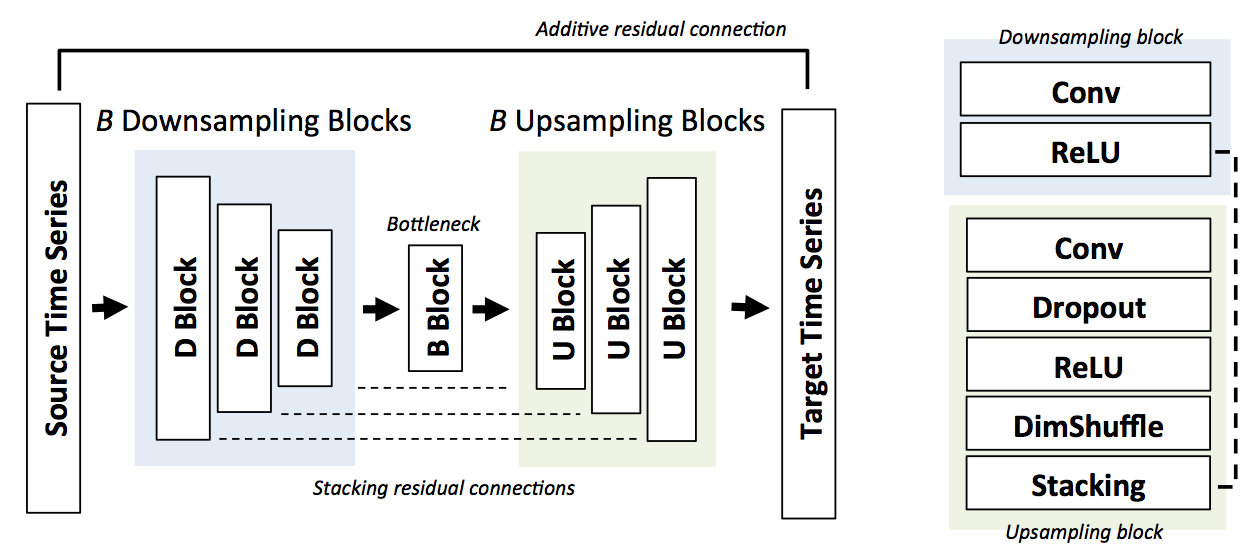
\includegraphics[scale=0.35]{img/audiounet.png}
		\captionsetup{margin=2cm}
		\caption{AudioUNet architecture. It consists of B successive downsampling/upsampling blocks linked by residual connections. From \cite{kuleshov2017audio}.}
		\label{fig:audiounet}
	\end{center}
\end{figure}
\noindent Figure ~\ref{fig:tfnet_pipeline} clearly illustrates that AudioUNet is used to model both the audio reconstruction and the spectral magnitude. It is important to indicate that B (the number of upsampling and downsampling blocks) is equal to 4 in both time and spectral branches. \\
As for the terminology used by Lim, Yeh \textit{et al.}, the term “Slim AudioUNet” in Fig. ~\ref{fig:tfnet_pipeline} refers to the fact that they reduce the original dimension of the network by halving the number of filters in each of the branch. Otherwise, the model is equal to the one just described.

\subsection{Spectral Replicator} \label{spectral_replicator}
As mentioned previously, the problem of audio \gls{sr} is based on the hypothesis that it is possible to reconstruct the high-frequency content of a signal from its corresponding low-frequency counterpart. The Spectral Replicator is a layer designed in order to alter the content of an input spectrum such that this low-high frequency dependency is explicitly expressed. The idea behind the design of this component is described in detail below. \\
Given that the objective of the system is to increase the sampling rate of a signal, it must be taken into account that, due to the Nyquist limit, there are some frequency components in the \gls{hr} target that can not exist in the \gls{lr} input sequence. It is possible to explain this concept formally in the following way. \\
Recalling the notation introduced in paragraph \ref{problem_formulation}, suppose we are trying to increase the temporal resolution of a signal $x$ sampled at $R_1$ by a factor of $r$. From the \gls{dsp} theory, we know that the Nyquist rate for that signal is equal to $R_{1_{lim}} = \frac{R_1}{2}$. However, the theoretical limit frequency of the \gls{hr} sequence is equal to $R_{2_{lim}} = r \times R_1$. From this point of view, audio \gls{sr} problem can be seen as the task of estimating the missing frequency components between $R_{1_{lim}}$ and $R_{2_{lim}}$. In other words, the aim of the system is to reconstruct the values over the interval $\interval{R_{1_{lim}}}{R_{2_{lim}}}$, on which the spectrum of the \gls{lr} sequence is null. \\
As mentioned extensively in the previous section, the reconstruction is made by a convolutional approach. Here arises a problem, since convolution is a local operation, i.e. only short-range dependencies in sequential inputs can be captured and processed due to the receptive field limitation. In other words, convolution cannot fully investigate non-local joint dependencies that could be useful to estimate the \gls{hr} spectrum. Therefore, it can be too challenging for a fully convolutional model to make the output’s high frequency component depend on the input’s low frequency counterpart. This limitation is accentuated as the scaling ratio $r$ increases, because the interval $\interval{R_{1_{lim}}}{R_{2_{lim}}}$ gets larger. \\
To overcome this issue, the Spectral Replicator layer explicitly replicates $r - 1$ times the low-frequency part of the signal, compensating the limitations of convolutional approaches. Therefore, all the zeros in the high frequency components of the spectrum are replaced by copies of the low frequency respective counterpart.\\
Specifically, each frequency term $k_i \in \interval{k_1}{k_{\frac{T_1}{2}}}$ (where $T_1$ is the length of $x$) is copied $r$ times through this layer. The only exception is given by the term $k_0$ (DC component), that, as said before, is not processed through the Spectral Replicator. \\
For example, suppose to have a signal $x$ whose spectral content is limited by the frequency term $k_{1024}$. For $4\times$ upsampling, we replace the zeros over the interval $\interval{k_{1025}}{k_{4096}}$ by repeating the 1st component to the 1024th one at 1025 to 2048, 2049 to 3072 and finally 3073 to 4096. Finally, these 4096 values are concatenated with the $k_0$ term. \\
Figure ~\ref{fig:spectral_replicator} illustrates the Spectral Replicator layer working on the \gls{bwe} task with $r = 4$. The input signal $x$ in the example has a sampling frequency of $R_1 =$ 8kHz, so that the Nyquist limit is $R_{1_{lim}} =$ 4kHz. As we can see, the low frequency patterns are replicated multiple times such that the zeros are replaced. \\
\begin{figure}[!htb]
	\begin{center}
		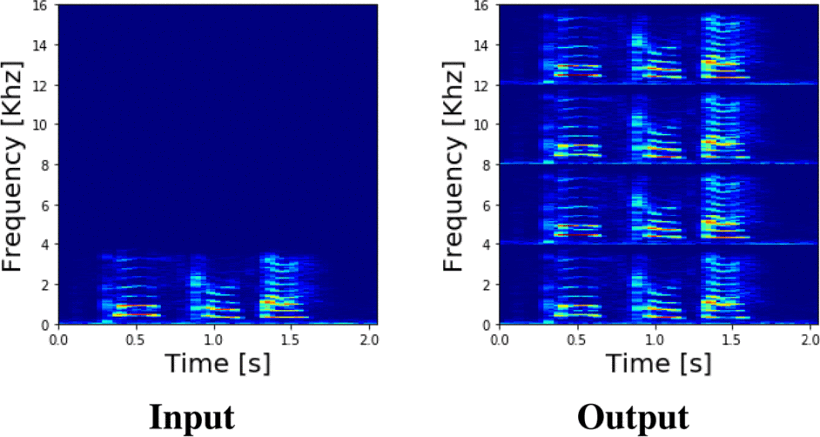
\includegraphics[scale=0.65]{img/spectral_replicator.png}
		\captionsetup{margin=2cm}
		\caption{Spectrogram showing how the signal is processed through the Spectral Replicator layer. The low-frequency components of the input spectrum are replicated three times in order to replace zeros in the high-frequency counterpart. From \cite{lim2018time}.}
		\label{fig:spectral_replicator}
	\end{center}
\end{figure} 
\subsection{Spectral Fusion Layer}
The spectral Fusion Layer is a key component of the \gls{tfnet} architecture. It permits to combine outputs of the two branches, i.e. $\hat{m}$ and $\hat{z}$, in a single \gls{hr} final reconstruction. To recap, the model predicts, for a given \gls{lr} input $x$, the estimation of the \gls{hr} audio reconstruction $\hat{z}$, and the \gls{hr} spectral magnitude $\hat{m}$. These two quantities are finally synthesized in the temporal domain through this layer. \\
Specifically, the process through which this happens consists of two main stages. First of all, since the two branches operate in two different domains, there is the need to reduce the data to the same domain. This operation is performed according to the following equation, which defines the \gls{hr} spectral magnitude estimate. 
\begin{align}\label{eq:spectralfusion1}
	\begin{array}{c}
		M=w \odot|\mathscr{F}(\hat{z})|+(1-w) \odot \hat{m}
	\end{array}
\end{align}
Equation ~\ref{eq:spectralfusion1} shows that the final estimation of the \gls{hr} spectral magnitude is a weighted average of the individual estimates provided by each branch. A data-driven approach is used to establish the weight of each branch in this operation. Indeed, this equation involves an element-wise multiplication with the trainable parameter $w$. \\
The second stage consists in calculating the final output $\hat{y}$ through Equation ~\ref{eq:spectralfusion2}. This one, is used to bring back the data to the original domain, i.e. the temporal one. Moreover, this second equation shows that the \gls{hr} phase is estimated only in the time domain.
\begin{align}\label{eq:spectralfusion2}
	\begin{array}{c}
		\hat{y}=\mathscr{F}^{-1}\left(M e^{j \angle \mathscr{F}(\hat{z})}\right)
	\end{array}
\end{align}
The Spectral Fusion Layer is fully differentiable and can be trained end-to-end.

\section{TFiLM} \label{tfilm}
The main objective of this paragraph is to present Temporal Feature-Wise Linear Modulation, a neural network component proposed by Birnbaum, Kuleshov \textit{et al.} in 2019 \cite{birnbaum2019temporal}. The key contribution of their work is to show that it is possible to capture long-term information in sequential inputs by combining elements of convolutional and recurrent approaches. \\
The main intuition behind the \gls{tfilm} approach is as follows. \gls{cnn}s, which are extensively used for audio \gls{sr}, can effectively process digital signals, such as audio, images or video and are relatively easy to train. However, these models have some disadvantages that could limit their prediction performance. In particular, convolutional approaches are not well suited for long sequential data processing because of the limited receptive field, which results in insufficient capacity to capture long-range input dependencies. Indeed, the larger the receptive field, the more a convolutional model is computationally complex. To overcome this issue, the researchers propose a particular architectural component that can capture both short and long-term interactions between features.\\
In summary, the \gls{tfilm} algorithm can be viewed as a temporal adaptive normalization layer that modulates the activations of a convolutional layer through a \gls{rnn}. More specifically, this algorithm takes as input a tensor of 1D multichannel convolutional activations $F \in \mathbf{R}^{T \times C}$ where $T, C$ are, respectively, the temporal dimension and the number of channels, and a positive integer value $B \in \mathbf{N}^{+}$ that identifies the block length. The output is an adaptively normalized tensor of activations $F' \in \mathbf{R}^{T \times C}$. The whole algorithm pipeline can be divided into five steps:
\begin{enumerate}
	\item Reshape $F$, along the spatial dimension, into a block tensor $F^{\mathrm{blk}} \in \mathbf{R}^{B \times T / B \times C},$ defined as $F_{b, t, c}^{\mathrm{blk}}=F_{b \times B+t, c}$. Each block can be considered as a region along the time axis in which the audio samples are closely correlated; for example, when processing audio, blocks could reasonably correspond to a set of activations that define a possible phoneme. 
	\item Obtain a representation $F^{\text {pool }} \in \mathbf{R}^{B \times C}$ of the block tensor by pooling together the channels within each block: $F_{b, c}^{\mathrm{pool}}=\operatorname{Pool}\left(F_{b,:, c}^{\mathrm{blk}}\right)$.
	\item  Compute, for $b=1,2, \ldots, B$, an affine transformation $\left(\gamma_{b}, \beta_{b}\right), h_{b}=\operatorname{RNN}\left(F_{b, \cdot}^{\text {pool }} ; h_{b-1}\right)$ using an \gls{rnn} applied to pooled blocks. The first value is $h_{0}=\overrightarrow{0}$, where $h_b$ denotes the hidden state and $\left(\gamma_{b}, \beta_{b}\right)$ is a tuple of trainable parameters. 
	\item Activations in each block b are normalized by $\gamma_{b}, \beta_{b}$. Formally, normalized block tensor $F^{\text {norm }} \in \mathbf{R}^{B \times T / B \times C}$ are computed as $F_{b, t, c}^{\text {norm }}=\gamma_{b, c} \cdot F_{b, t, c}^{\text {block }}+\beta_{b, c}$.
	\item Reshape $F^{\text {norm }}$ into output $F^{\prime} \in \mathbf{R}^{T \times C}$ as $F_{\ell, c}^{\prime}=F_{\lfloor t / B\rfloor, t \bmod B, c}^{\text {norm }}$.
\end{enumerate}               
                      
\noindent Notice that the way through which activations are modulated using long-range input dependencies is well described in the third stage. Indeed, we can see that each $\gamma_{b}, \beta_{b}$ is a function of both the current and all the past blocks. By doing so, all long-term informations are captured by the \gls{rnn} and processed for each hidden state. To better understand the main idea behind \gls{film}, see paragraph \ref{film}. \\
The main features of this architectural component are illustrated in Fig. ~\ref{fig:tflim_layer}. It is important to underline that, although the image illustrates a \gls{bilstm} network, actually a unidirectional \gls{lstm} is used. Researchers in the paper perform several experiments with the specific aim to investigate the impact of using bidirectional \gls{rnn}s rather than standard unidirectional recurrent layers. Their results show that, generally, switching from a unidirectional \gls{lstm} to a \gls{bilstm} does not provide a significant improvement in performance and, in some cases, it even increase the prediction error (perhaps due to overfitting). Moreover, there is a remarkable saving in computational power cost by using unidirectional recurrent approaches. \\
This layer efficiently incorporates long-term information when processing sequential data. \\                                       
\begin{figure}[H]                                   
	\begin{center}                                     
		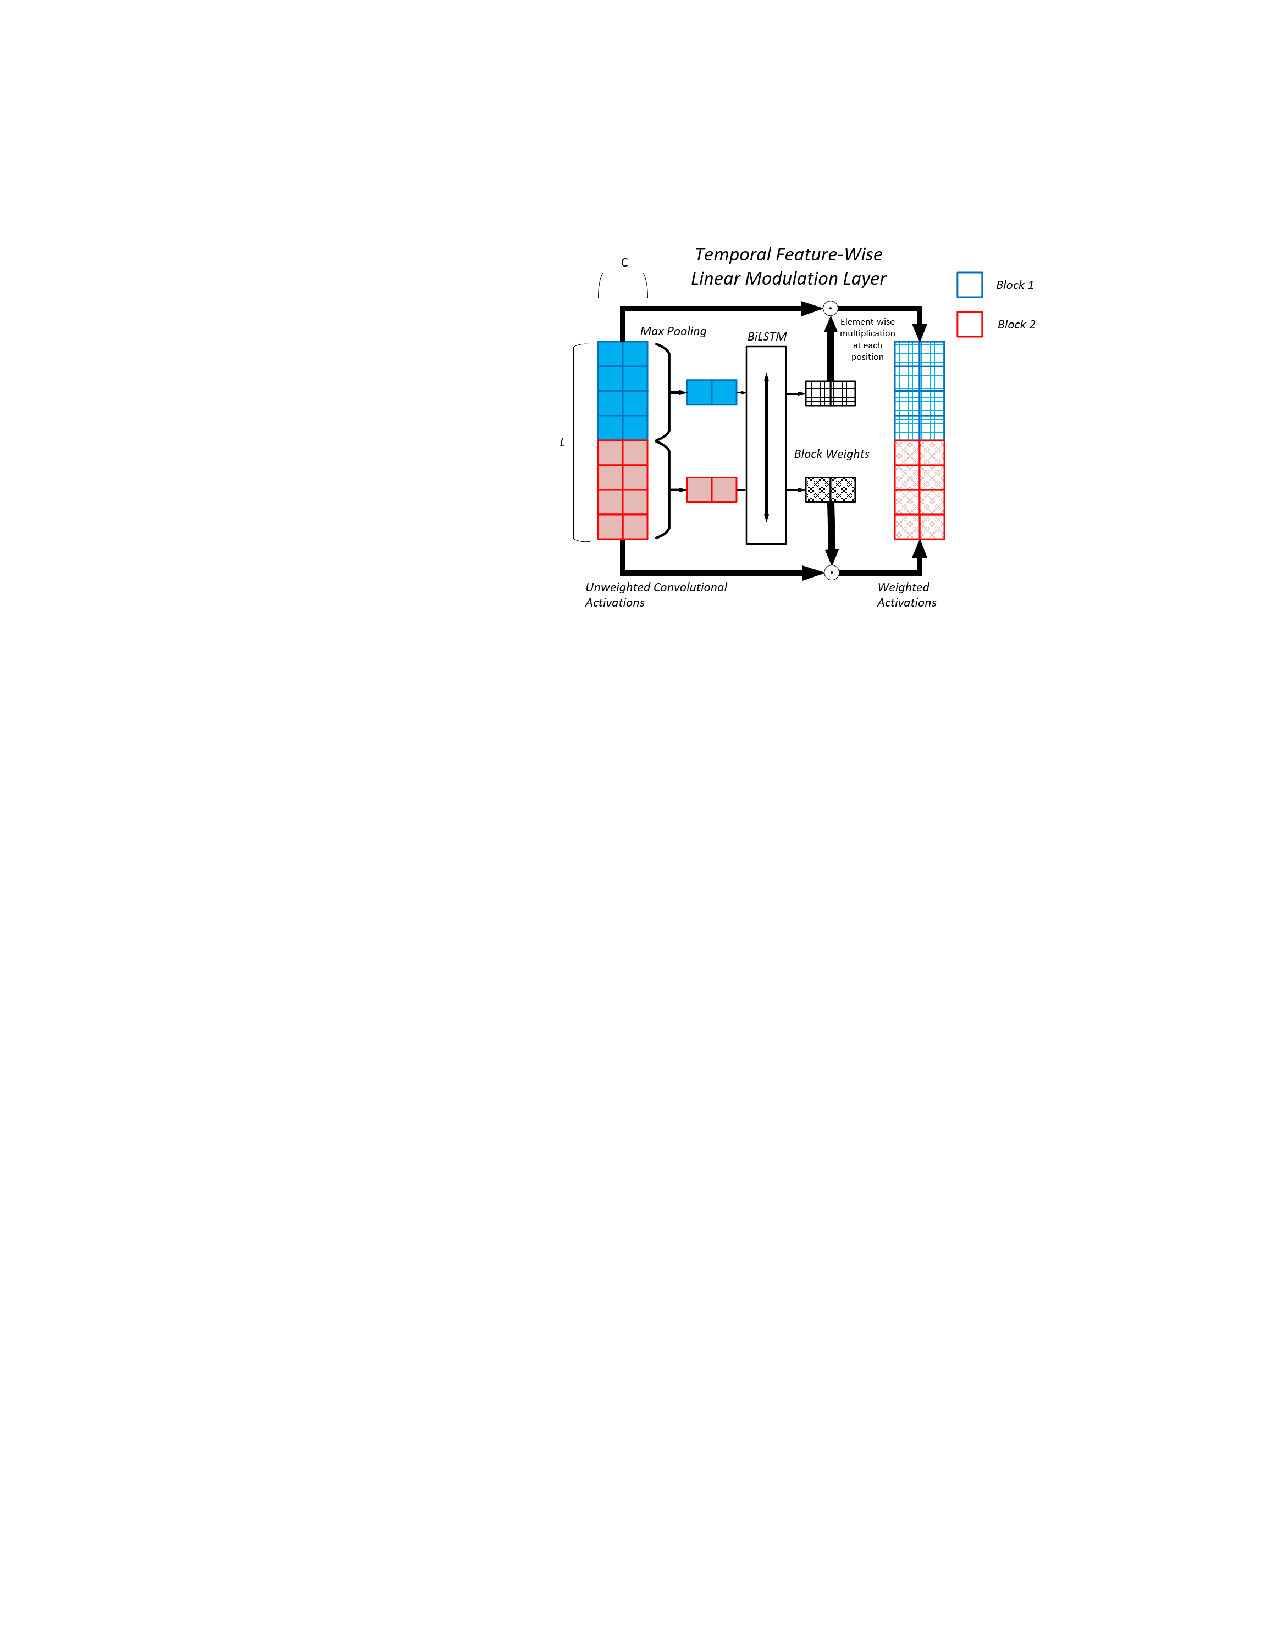
\includegraphics[scale=1.5]{img/tfilm_layer.pdf}  
		\captionsetup{margin=2cm}                         
		\caption{The \gls{tfilm} layer in detail. In this example the 1D tensor of convolutional activations has the following shape: $F \in \mathbf{R}^{8 \times 2}$. The 2 blocks are first processed by a Max Pooling layer (whit a pooling factor of 2) and then by the \gls{rnn}. Finally, the output of the recurrent network is used to modulate the convolutional layer.From \cite{birnbaum2019temporal}.}
		\label{fig:tflim_layer}                           
	\end{center}                                       
\end{figure}                                        
\noindent A significant difference between \gls{tfnet} and \gls{tfilm} lies in the fact that, while the former architecture is domain-dependent, the latter is domain-agnostic. Indeed, \gls{tfnet} performs domain-specific operations on signals such as \gls{dft}, while \gls{tfilm} layer does not require any of these operations. This fact has made the application of this model possible with regard to a wide variety of tasks. In general, \gls{tfilm} can be useful to process any sequential data. In fact, in the paper, the model’s effectiveness is demonstrated on three diverse domains: Text Classification, Audio \gls{sr} and Chromatin Immunoprecipitation Sequencing. The latter is a particular genomic experiment that consists in reconstructing high-quality measurements taken using a large set of probes (e.g., sequencing reads) from noisy measurements taken using a small set of probes. \\
It is interesting to point out that, for the researchers, Audio \gls{sr} and Chromatin Immunoprecipitation Sequencing tasks belong to the same class of generative modeling tasks, called \textit{time series super-resolution}. This problem consists in reconstructing a \gls{hr} signal from \gls{lr} measurements. \\
A brief overview of the model architecture proposed for time-series \gls{sr} tasks is given in Figure ~\ref{fig:tflim_architecture}. We can call this model \gls{tfilm} Net. \\
\begin{figure}[H]
	\begin{center}
		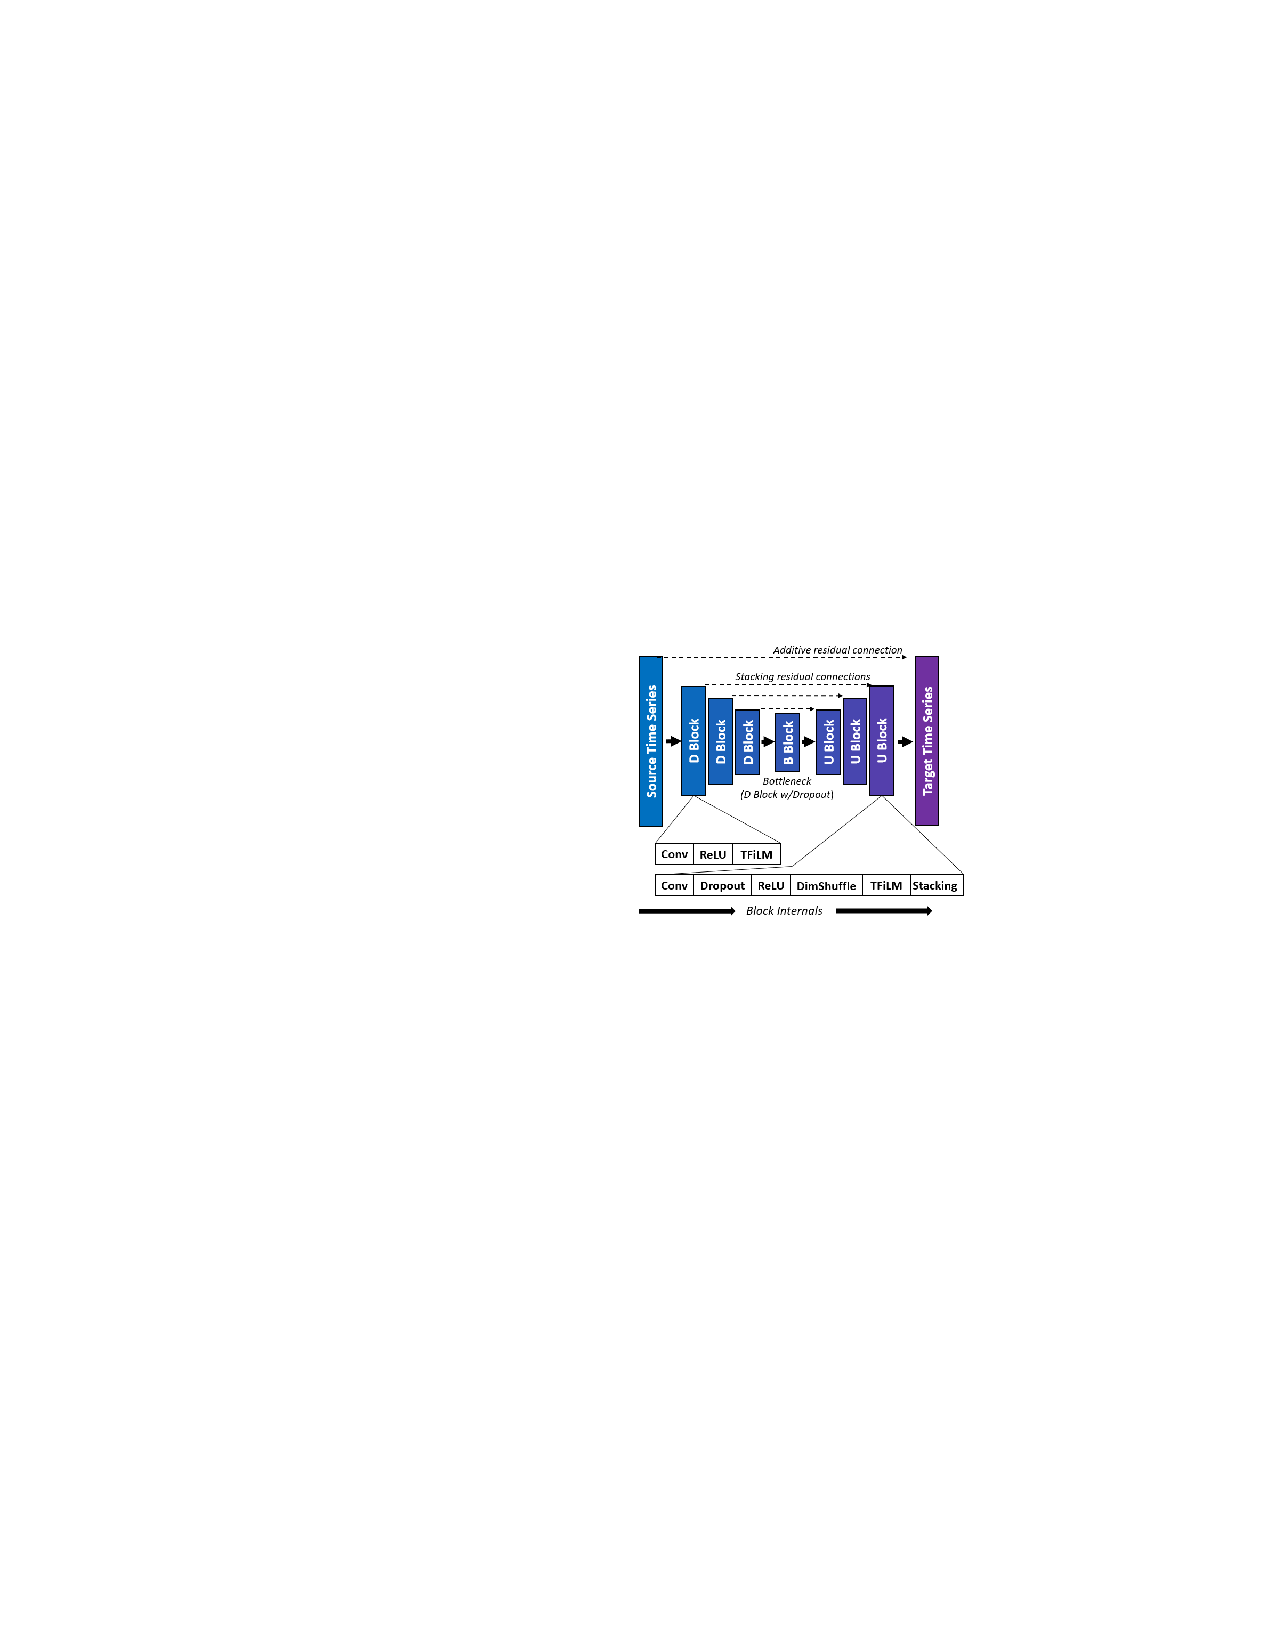
\includegraphics[scale=1.9]{img/tfilm_bottleneck.pdf}
		\captionsetup{margin=2cm}
		\caption{\textit{Top}: \gls{tfilm} Net architecture used for audio super-resolution. It consists of K downsampling blocks followed by a bottleneck layer and K upsampling blocks; features are reused via symmetric residual skip connections. \textit{Bottom}: Internal structure of downsampling and upsampling convolutional blocks. From \cite{birnbaum2019temporal}.}
		\label{fig:tflim_architecture}
	\end{center}
\end{figure}
\noindent As we can see, the architecture of \gls{tfilm} Net follows design patterns of AudioUNet (described in ~\ref{audiounet}). Indeed, we can recognize the bottleneck architecture, the subpixel layer, the use of B successive upsampling/downsampling blocks and the adoption of residual connections. This is not surprising because three of the authors are the same for both articles (i.e. \cite{kuleshov2017audio}, \cite{birnbaum2019temporal}).\\
However, there are several differences between AudioUNet and \gls{tfilm} Net, such as the use of recurrent and Feature-Wise Linear Modulation layers. Moreover, while AudioUNet uses standard convolutional layers, \gls{tfilm} Net exploits dilated convolutional approaches to extract highly representative features from a wider receptive field. Dilated convolution is described in detail in section ~\ref{dilated_conv}. \\
As for implementation details, it is essential to note that the authors instantiated the model with $K = 4$ (recalling that $K$ is the number of  upsampling and downsampling blocks). Another important hyperparameter is the number of \gls{tfilm} layer blocks $L = \frac{T}{B}$. In this regard, the block length values $B$ are adjusted for each layer so that the ratio between the temporal dimension $T$ and $B$ is always 32. In other words, the number of blocks $L$ is set to 32 in each \gls{tfilm} layer. \\
In order to facilitate understanding of the whole process, a graphical representation of the entire entire pipeline of \gls{tfilm} Net is proposed in Figure ~\ref{fig:tfilm_pipeline}. \\
\begin{figure}[!htb]
	\begin{center}
		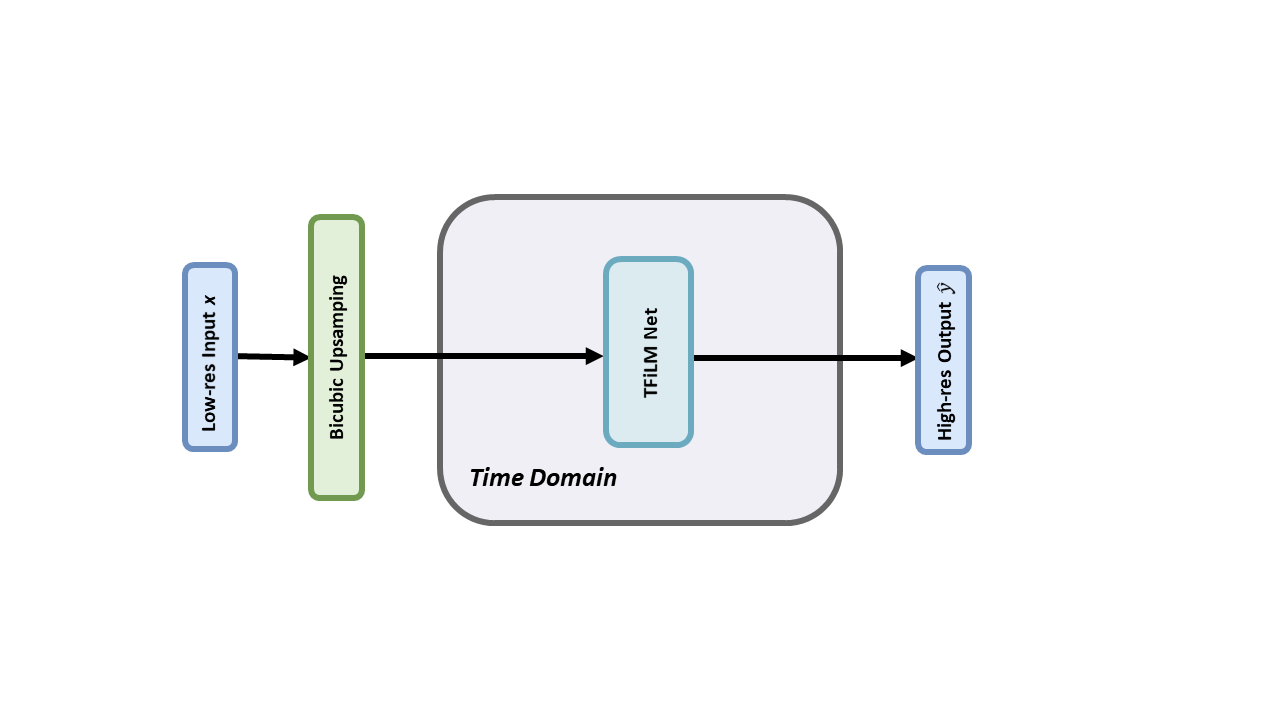
\includegraphics[scale=0.48]{img/tfilm_pipeline.png}
		\captionsetup{margin=2cm}
		\caption{Overall pipeline of \gls{tfilm} Net. The system integrates convolutional and recurrent layers to efficiently incorporate long-term input dependencies by operating in the time-domain.} 
		\label{fig:tfilm_pipeline}
	\end{center}
\end{figure}


\subsection{Dilated Convolution} \label{dilated_conv}
\noindent To further increase the receptive field of convolutional layers, authors use dilated convolutions with a dilation factor of 2. \\
Dilated convolution \cite{yu2015multi} is a generalization of the familiar discrete-convolution (that can be considered as the 1-dilated convolution). In summary, this particular type of convolution, defines a spacing between the values in a kernel. This allows to increase the receptive field of a convolution, without a corresponding increase in the number of trainable parameters. Therefore, the choice to use this type of layer is perfectly consistent with the objectives of this work.\\
For example, considering the two-dimensional convolution, a $3 \times 3$ kernel with a dilation rate of 2 results to have the same receptive field of view as a $7 \times 7$ kernel. A graphical representation of this example is provided in Figure ~\ref{fig:dilated_conv}.

\begin{figure}[H]
	\begin{center}
		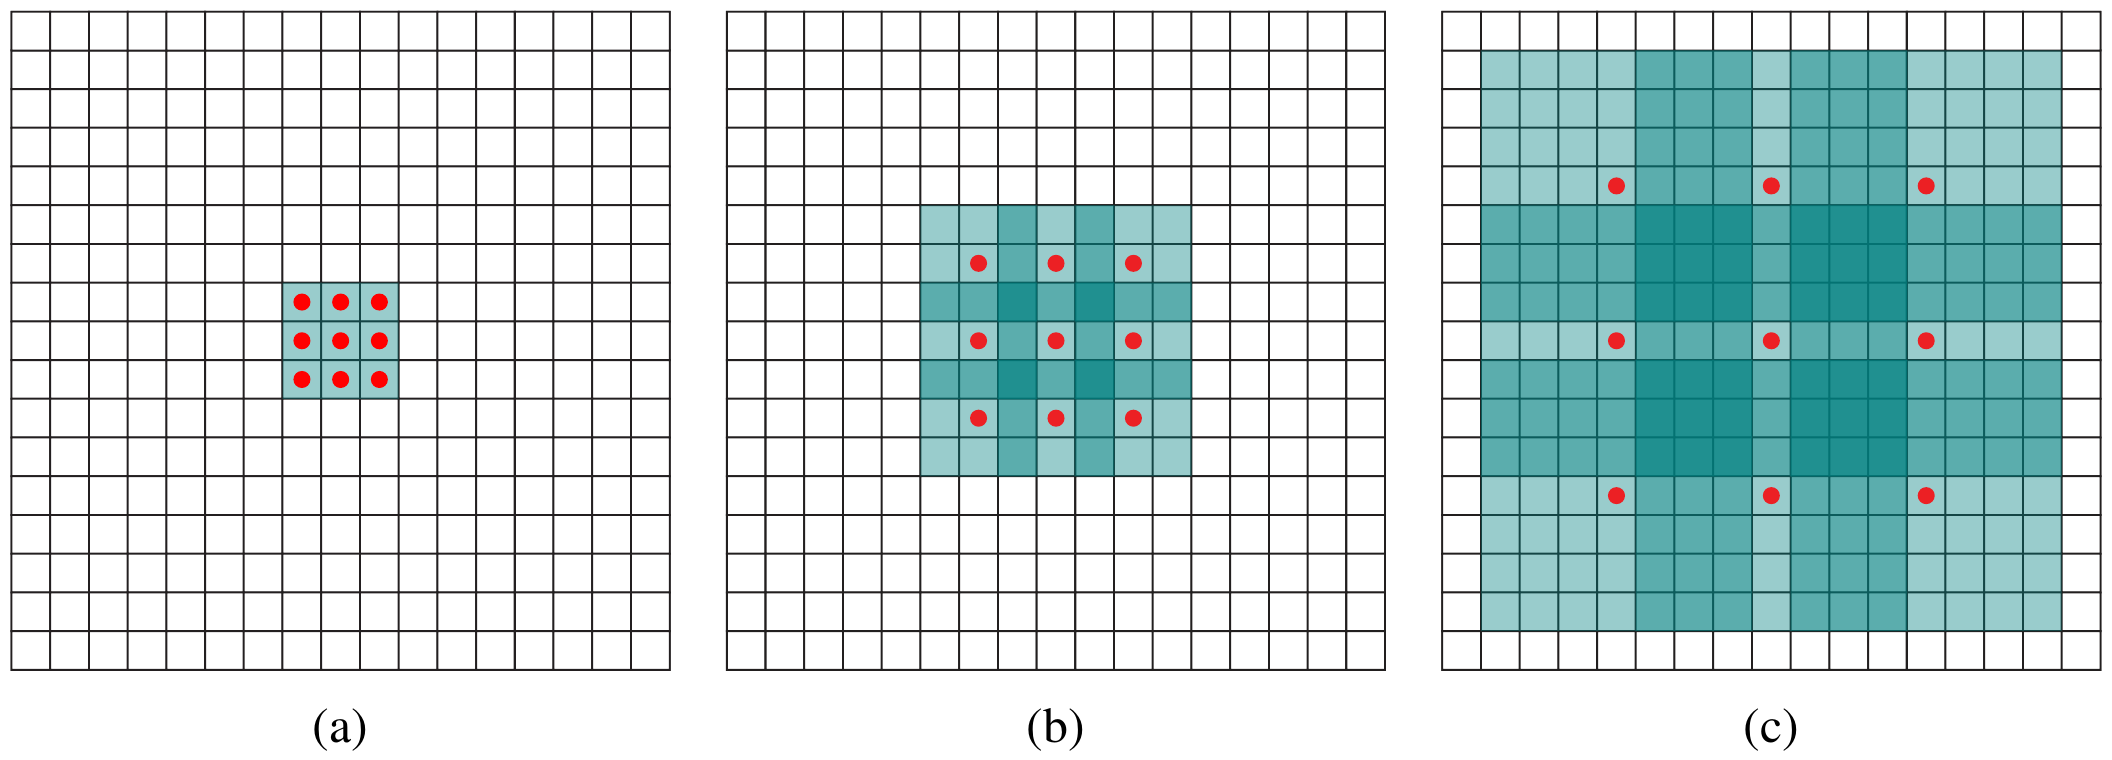
\includegraphics[scale=.21]{img/dilated_conv.png}
		\captionsetup{margin=2cm}
		\caption{(a) 1-Dilated Convolution has a receptive field of $3 \times 3$. (b) 2-Dilated Convolution has a receptive field of $7 \times 7$. (c) 4-Dilated Convolution has a receptive field of $15 \times 15$. The number of parameters associated with each layer is identical. The receptive field grows exponentially while the number of parameters grows linearly. From \cite{yu2015multi}.}
		\label{fig:dilated_conv}
	\end{center}
\end{figure}

\subsection{Feature-Wise Linear Modulation} \label{film}
As the name suggests, a \gls{film} layer applies a feature-wise affine transformation, based on conditioning informations of an auxiliary input $z \in \mathbf{Z}$. \gls{film} can be thought of as a generalization of Conditional Normalization \cite{dumoulin2016learned}, that is used in \gls{dl} for stabilizing the training of the models. Batch Normalization and \gls{film} are formally described as follows. \\
Consider a tensor of 1D multichannel convolutional activations $F \in \mathbf{R}^{T \times C}$ (where $T$ is the time axis and $C$ is equal to the number of channels). The batch normalization  rescales $F$ and applies an affine transformation, so that it produces an output $F^{\prime} \in \mathbf{R}^{T \times C}$ whose $(t, c)$ -th output elements are described in Equation \ref{eq:batch_norm}:
\begin{align}\label{eq:batch_norm}
	\begin{array}{c}
		F_{t, c}^{\prime}=\gamma_{c} \hat{F}_{t, c}+\beta_{c}
	\end{array}
\end{align}
Where $\hat{F}_{t, c}$ is defined as follows.
\begin{align}\label{eq:batch_norm2}
	\begin{array}{c}
		\hat{F}_{t, c}=\frac{F_{t, c}-\mu_{c}}{\sigma_{c}+\epsilon} 
	\end{array}
\end{align}
From the notational point of view, it is important to define $\mu_{c}, \sigma_{c}$ that are, respectively, the estimates of the mean and standard deviation for the $c$ -th channel. As for $\gamma, \beta \in \mathbf{R}^{C}$, they are trainable parameters. \\
\gls{film} \cite{perez2018film} extends this idea by allowing $\gamma, \beta$ to be functions $\gamma, \beta: \mathcal{Z} \rightarrow \mathbf{R}^{C}$ of an auxiliary input $z \in \mathcal{Z}$. This technique is domain independent, i.e. can be used for a wide variety of applications. For example, in feed-forward image style transfer \cite{dumoulin2016learned}, $z$ is an image defining a new style; by using different $\gamma(z), \beta(z)$ for each $z$, the same feed-forward network (using the same weights) can apply different styles to a target image. \gls{film} has also obtained significant results in speech recognition \cite{kim2017dynamic} and image classification \cite{hu2018squeeze}. 

\section{Proposed Model Architecture}
The main objective of this paragraph is to provide a detailed explanation of the proposed model, that aims to combine elements of both \gls{tfnet} and \gls{tfilm} Net in an effective way.\\
Taking inspiration from \gls{tfnet}, the proposed deep network architecture is made of two branches: one for time-domain and one for spectral-domain processing. Indeed, Lim, Yeh \textit{et al.} demonstrate that this strategy helps the model to better estimate the high-frequency content of the signal. However, their approach is fully convolutional. In this regard, Birnbaum, Kuleshov \textit{et al.} highlight that \gls{cnn}-based methods have intrinsic limitations when applied to sequential data. As mentioned before, \gls{cnn}s are not effective for capturing long-term dependency due to the relatively high computational requirements of large receptive fields. To address this problem, the proposed model incorporates \gls{tfilm} components in the processing. More specifically, the AudioUNet components used in \gls{tfnet} are replaced with the \gls{tfilm} layers, that can capture long-range input dependencies by modulating the activations of a convolutional layer through a \gls{rnn}. \\
To further capture the low-high frequency dependency in the signal, it is decided to keep the spectral replicator layer in the model architecture. It would also be interesting to evaluate the impact of this operation by training another model that does not have this layer in its pipeline.
\\ To sum up, the proposed approach mainly aims to overcome the limitations of the \gls{tfnet} architecture, with which it shares a similar pipeline. Indeed, key components, such as the Spectral Replicator and the Spectral Fusion Layer, are maintained in the system. \\
A graphical representation of the model pipeline is provided in Figure ~\ref{fig:proposed_pipeline}. \\
From a notational point of view, the term "Slim \gls{tfilm} Net" indicates that the original dimension of the network is reduced by halving the number of filters in each branch. \\
The Slim \gls{tfilm} Nets in the two branches are dimensionally equivalent: both the size and the number of filters applied in each layer are the same. What changes is the length of the input sequence. Indeed, as in the case of \gls{tfnet} model, a \gls{dft} on the sequence is computed to pass from the time to the spectral domain. Because of this, the spectral branch processes a signal that is half the length of the time branch signal.  
\begin{figure}[!htb]
	\begin{center}
		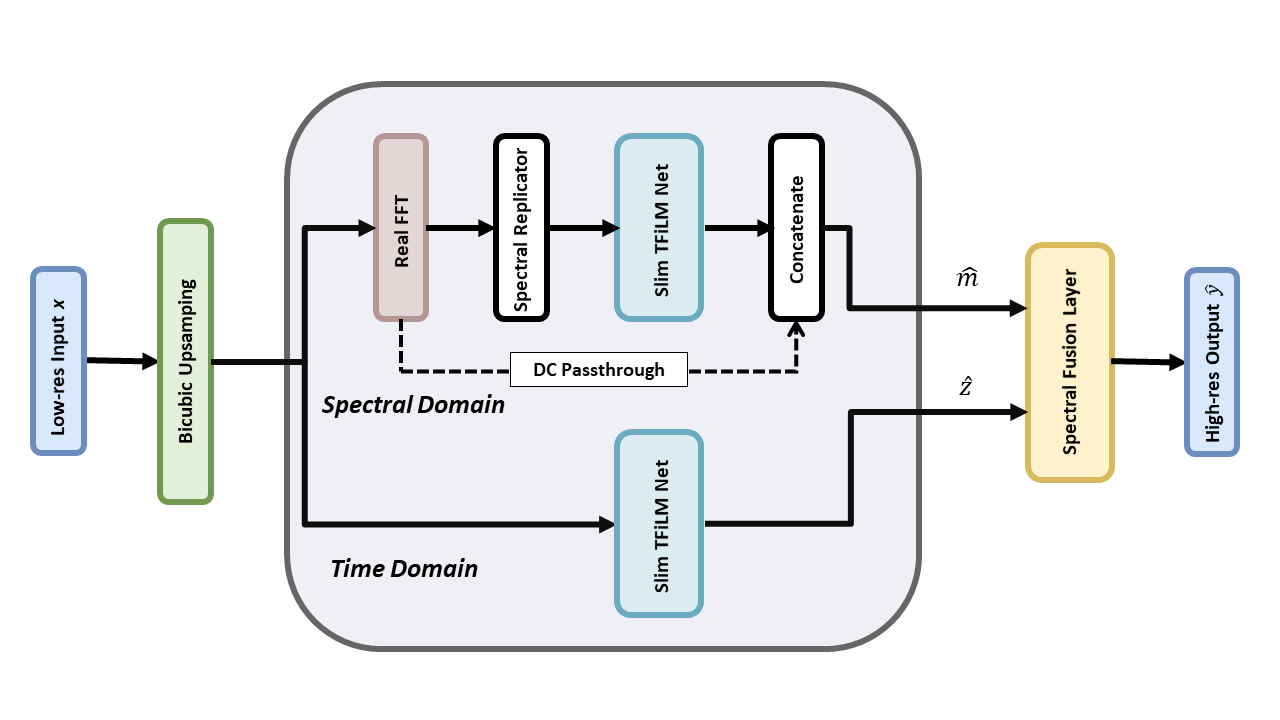
\includegraphics[scale=0.48]{img/proposed_pipeline.png}
		\captionsetup{margin=2cm}
		\caption{Overall pipeline of the proposed model. On one hand, the system maintains the branching structure of \gls{tfnet} that allows to processes audio in both time and frequency domain. On the other hand, the model uses \gls{tfilm} Net to predict both the audio reconstruction and the spectral magnitude.} 
		\label{fig:proposed_pipeline}
	\end{center}
\end{figure}


\section{Implementation details} \label{implementation_details}
As mentioned earlier, in order to identify which is the best architecture between different models, it is important to establish a context that is as fair as possible for the comparison. In this sense, the number of trainable parameters can serve as a benchmark criterion for comparing different results. \\ Here, however, there is a problem. The available computational resources do not allow to propose and train a model with the same dimensions of \gls{tfnet} and \gls{tfilm} Net. In fact, these two models have roughly 35M parameters, while the available resources allow to train models with approximately 22M parameters. This gap is too wide to compare the results reported in the papers \cite{lim2018time}, \cite{birnbaum2019temporal} with the novel model architecture. For this reason, it is decided to reduce the dimensionality and re-train both \gls{tfnet} and \gls{tfilm} Net. \\
To achieve this goal, we proceed in the following way. Recalling that the \gls{dl} components of the models, i.e. AudioUNet and \gls{tfilm}, have a bottleneck architecture that consists of downsampling and upsampling blocks, it is decided to remove the last layer (which is the largest) from all of these components. By doing so, the number of upsampling and downsampling blocks (called B in \ref{audiounet} and K in \ref{tfilm}) is reduced from 4 to 3.\\
This change is enough to enable the model training within the computational limits available to us. Therefore, all other architectural characteristics of the models remain faithful to the original implementation.\\
Another difference from the papers \cite{lim2018time}, \cite{birnbaum2019temporal} concerns the data used for the training: the dataset is the same as the one used in both papers, but in this project we sample a subset of recordings because of dimensionality issues. This is explained in more details in Chapter \ref{chap:exp_results}. 

